\section{Gestión de Tareas}
    \subsection{Consulta de Tareas}
        El usuario tendrá a su disposición 2 funciones para la gestion de tareas:

	    \subsection{Asignar Tarea}

        	Para ello, el usuario tendrá que dar clic en el botón con el icono de una tablita que esta en la fila de la Unidad de Aprendizaje indicada.

            \begin{figure}[H]
                \centering
                \hypertarget{boton}{
\includegraphics[width=0.7\linewidth]{images/Tarea/boton}}
                \caption{Botón Asignar}
                \label{boton}
            \end{figure}

            Al hacer esto, el sistema redireccionará al usuario a la pantalla siguiente donde podrá seleccionar un usuario para asignarle una tarea.
            
            \begin{figure}[H]
                \centering
                \hypertarget{asigna}{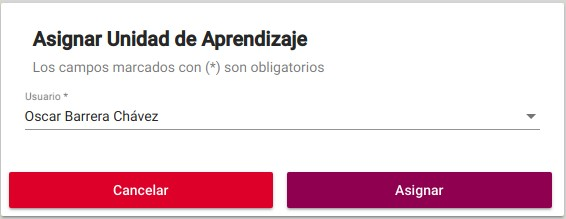
\includegraphics[width=0.7\linewidth]{images/Tarea/Asignando}}
                \caption{Seleccion de usuario para tarea}
                \label{asigna}
            \end{figure}

            Si el usuario desea agregar mas usuarios solo da click en el boton Asignar y le mostrará el siguiente mensaje.
            \begin{figure}[H]
                \centering
                \hypertarget{asignar}{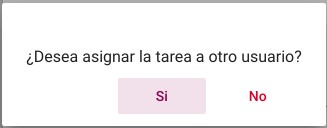
\includegraphics[width=0.7\linewidth]{images/Tarea/Asignarotro}}
                \caption{Seleccion de otro usuario}
                \label{asignar}
            \end{figure}

   
        \subsection{Consultar Tarea}

            El usuario podrá ver una tabla con todas las tareas relacionadas a él.

            \begin{figure}[H]
                \centering
                \hypertarget{asignart}{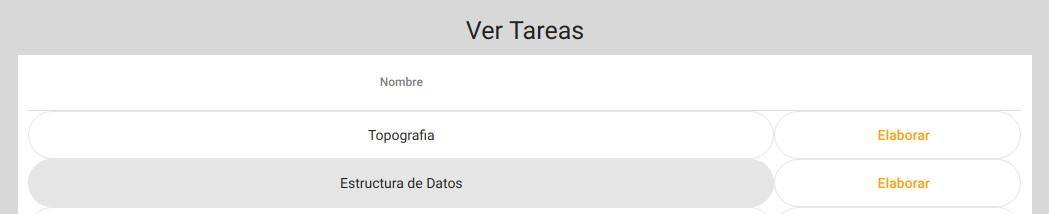
\includegraphics[width=0.7\linewidth]{images/Tarea/Vertareas}}
                \caption{Tabla de tareas}
                \label{asignart}
            \end{figure}

   